%title:
%improving 2DoF pixel-based image synthesis of 360deg viewpoints using flow-based interpolation
%2DoF pixel-based synthesis of 360deg viewpoints using flow-based interpolation
%2 degree of freedom pixel-based synthesis of 360deg viewpoints with flow-based interpolation
%pixel-based synthesis of 360\degree viewpoints using flow-based interpolation
\chapter{Introduction}

Over the past decade, Virtual Reality (VR) technology has experienced a resurgence in popularity due to the development of a number of affordable, consumer-quality head-mounted displays\footnote{The price of a consumer-quality VR headset is between approximately 20 and 1000 USD as of January 2021, including headsets for use with a smartphone (\url{https://www.tomsguide.com/us/best-vr-headsets,review-3550.html}, \emph{accessed Jan 13, 2021})}. These displays allow a user to experience and interact with a virtual environment in 3D, for example by playing games, or by taking virtual tours of cities, historical landmarks, or remote locations in nature.
%\footnote{``10 of the best virtual reality travel experiences'', Paul Joseph, Travelmag (\url{https://www.travelmag.com/articles/virtual-reality-travel-experiences/}, \emph{accessed Jan 13, 2021})}

Some of these environments are modeled meticulously in 3D, while others use 360\degree images taken at the locations. Often, the 3D-modeled environments allow a lot of freedom of movement, enabling the user to ``walk'' around and inspect elements of the scene at will. Unfortunately, modeling a real environment by hand to be viewed interactively requires an enormous amount of effort and even then it is very unlikely to achieve photo-realism. An alternative is to capture the location with a 360\degree camera, which records the entire surroundings in a single image. Viewing these images offers photo-realism (as they are actual photos), but often awkward navigation, for example forcing the user to ``jump'' from one image location to the next, instead of being able to ``walk'' smoothly around the scene. Nonetheless, the ease of capturing 360\degree images with modern 360\degree cameras, along with their significant advantage of photo-realism, makes this an attractive method for creating immersive VR environments.

The difficulties of navigating an environment captured by way of 360\degree cameras are not a new phenomenon. Virtual tours also exist outside of the realm of VR, viewed on regular computer or smartphone screens, for example interactive tours of museums, real-estate, or other locations of interest. A prominent example is Google's Street View, which allows users to navigate streets and monuments around the world by way of 360\degree images.

Whether a scene is viewed stereoscopically with a head-mounted display, or monoscopically on a flat screen, the greatest obstacle at the moment is the problem of interactive, user-driven navigation. Ideally, a user would be able to go anywhere they liked in the scene, and view anything they wanted from any angle and at any level of detail. Unfortunately, for environments captured by way of a 360\degree camera, this type of interaction would require a prohibitive amount of data, as well as being impossible to manually execute, since a separate image would have to be captured at every possible viewing position.

An alternative to capturing all of these viewpoints manually is to generate them digitally. This requires capturing a much smaller subset of images and using these to generate the rest of the viewpoints. Generating new images based on already captured images is generally known as \emph{image-based rendering} (IBR), or image-based synthesis. There are many different approaches to synthesizing new images from captured ones, and they can generally be categorized by the area where new images can be synthesized, as well as the type and amount of information extracted from the captured images.
%degrees of freedom (DoF) that the technique can synthesize images with

The area and the degrees of freedom (DoF) that are necessary usually depend on the goal and requirements of the application: A virtual tour on a pre-defined path for example, would only require generating intermediate views between existing viewpoints (i.e.\ synthesis with 1DoF) for a smooth transition. For a less constrained virtual tour that enables the user to navigate freely, generating viewpoints with 2DoF at eye-height could be sufficient. The user could move around and look in any direction but not change their viewing height. Some applications may require three degrees of freedom, for example in order to enable the user to closely inspect certain objects from all angles, but restrict them from moving away from the object.

Depending on the type of scene, the required fidelity, and real-time requirements, different IBR techniques leverage different amounts and types of information extracted from the input images. On one end of the scale, there are approaches that extract as much geometry information as possible from the set of images and try to reconstruct the 3D geometry of the scene as closely as possible. These approaches can suffer from the problem of extracting accurate geometry information, since errors in geometry can lead to unappealing results.
Then, there are approaches that try to extract some information from the image, such as feature correspondences, or motion vectors (optical flow), which enables interpolation between pairs of images, i.e.\ a smooth transition with 1DoF.
Approaches at the other end of the scale use no semantic image information whatsoever. They may use color values, simple proxies for the scene geometry, or information about the relative location of captures, but they tend to operate on pixel-level. There is no distinct name for this, so the term used in this thesis is \emph{pixel-based synthesis}.

One very basic form of pixel-based synthesis is to use a simple proxy (``stand-in'') geometry, for example a sphere, in place of the real scene geometry\footnotemark. This allows for resampling the captured images in order to create a new viewpoint any location within the scene, without having to estimate or record the actual scene geometry. However, the potentially drastic difference between the proxy and the actual geometry can lead to severe distortions and artefacts in the resampled images. Although this basic form of pixel-based rendering using proxy geometry may be unsuitable for scenes where the real geometry differs greatly from the proxy geometry, it may be possible to improve these results by combining the basic technique with a 1DoF interpolation method.
\footnotetext{The term ``proxy geometry'' is used in this thesis as a term for the model used in place of the real scene geometry. It can be anything from a simple geometric shape such as a sphere, to a simplified version of the real scene geometry}

\section*{Problem Statement}
A number of 1DoF interpolation techniques exist, many of them using some form of feature correspondence. Flow-based interpolation is one of these techniques that has already been used successfully for 360\degree images. It uses motion vectors (``optical flow'') between pairs of images to interpolate new viewpoints between them. The goal of this thesis is to answer the following research questions:

\begin{enumerate}
  \item Can flow-based interpolation be used in pixel-based synthesis with proxy geometry?
  \item If it can, does this improve the accuracy of the results?
\end{enumerate}

In order to measure the accuracy of the different results, the synthesized images are compared with the ground truth images using two different error metrics, as well as being assessed visually.
%Simple resampling with no geometry 
%Could flow-based interpolation improve the result of a basic resampling approach without scene geometry in 2DoF?
%improving 2DoF pixel-based image synthesis of 360deg viewpoints using flow-based interpolation
%- 1DoF with flow-based interpolation
%- 2DoF with resampling (and other approaches)
%(actually, 4/5 DoF, but rotation is not considered, since this is 360)


\section*{Scope}
The number of possible different environments is infinite, as well as the positions at which images can be captured. In order to reduce the parameter space for testing and evaluation, several restrictions are made. First of all, only indoor scenes are examined. The scenes are assumed to be static, meaning the objects within the scene do not change their positions. To reduce the complexity of the implementation, as well as the number of necessary input images to be captured, only 2DoF synthesis is considered. This means that all captured and synthesized viewpoints are located on a plane at approximate eye-height parallel to the ground. 

%fixed:
%  the scale (max radius) of the scene is known

The parameters that will be examined are:
\begin{description}
  \item[Density of captured viewpoints] For the evaluation in this thesis, the viewpoints used for synthesis (the ``captured viewpoints'') are arranged on a regular grid. The effect of different densities on the accuracy of the results is explored, specifically, grids of between 3m and 30cm distance are used.
  \item[Location of synthesized points relative to captured points] Since the captured viewpoints are arranged on a grid, there are many positions where a synthesized point can be on a line between two captured viewoints. In this case, the problem is reduced to 1DoF interpolation. This is compared to the case where the synthesized point is not located on any line, which requires 2DoF synthesis.
  \item[Difference between the scene geometry and the proxy geometry] The proxy geometry used in the approach is a sphere of the approximate size of the scene. Scenes of different shapes are tested, in order to gauge the effect of the difference between the proxy model and the scene. The ``difference'' of the model to the sphere is difficult to quantify in a meaningful way, so it is not measured but done intuitively. For example, a scene with the basic shape of a cube is more similar to a sphere than a narrow, long scene. Only simple basic scene shapes are examined, for example a spherical scene, a scene in the shape of a cube, and a scene in the shape of an oblong rectangular cuboid.
  \item[Location of synthesized points within the scene] Finally, the location of the synthesized points within the scene in relation to objects in the scene is examined. Again, this is difficult to quantify and will be done by synthesizing points regularly throughout the scene and visually comparing the error values to the proximity to different objects.
\end{description}

These parameters will not be examined exhaustively, as this is impossible, given the infinite possibilities of scene shapes and object placements, alone. Instead, for each parameter to be examined, a scenario is designed that tests this parameter in a reasonable context.

%Since the implementation is a basic proof-of-concept, a user study does not make much sense, since the results are expected to have some distinct artefacts. Instead, two mathematical error metrics are used to compare the 

%2DoF synthesis without geometry in indoor environments
%variable
%quantified:
%  the location of synthesized points relative to the captured points
%  density of captured viewpoints
%
%not quantified
%  effect of objects within the scene
%  scene - model difference
%  the location of synthesized points within the scene (near walls, objects, etc)
%
%  evaluation:
%    mathematical error metrics to compare result to ground truth: mean absolute error and ssim
%
%basic proof of concept implementation \ar not perfect, real-time
%not an exhaustive evaluation of all possible parameters \& combinations
%not a comparison to other implementations (missing benchmark data and implementation of other methods is outside of scope)
%
%will be evaluating following scenarios:
%Effect of Viewpoint Density
%Viewpoint Density and Choice of Viewpoints to be Synthesized
%Position of Synthesized Viewpoints Relative to Captured Viewpoints
%Effect of Different Scenes

\section*{Methodology}
In order to implement and evaluate an algorithm that combines basic pixel-based synthesis and flow-based interpolation, this thesis follows a methodology made up of two distinct phases: implementation and evaluation (Figure~\ref{fig:methodology}). The implementation consists of first developing a basic pixel-based synthesis algorithm using a proxy geometry. Then, based on existing 1DoF flow-based interpolation algorithms (presented in Section~\ref{sec:related_work}), the extended pixel-based algorithm using flow-based interpolation is developed. The approach and implementation are presented in Chapter~\ref{chap:implementation}.

The evaluation step is further divided into three phases. In the preparation phase, based on the parameter space described in detail in Section~\ref{sec:params}, data for testing and evaluation is acquired. This data includes virtual scenes rendered using animation software, and real scenes captured with a 360\degree camera. Additionally, the error metrics are adapted for 360\degree images (Section~\ref{sec:eval_methodology}).
Then, in the synthesis and testing phase, the images are synthesized using the implementations developed in the implementations step. Using the result images and the ground truth data generated during the data acquision, the error calculation is performed with the adapted metrics.
Finally, using the calculated error values, along with the synthesized images, the results are analyzed. The analysis is made up of two parts: First, an analysis is performed on the virtual data that explores the limits of the chosen parameters (Section~\ref{sec:limit_eval}). Then, the results using the real data are examined as a proof-of-concept (Section~\ref{sec:pof_eval}).

\begin{figure}
		\centering
		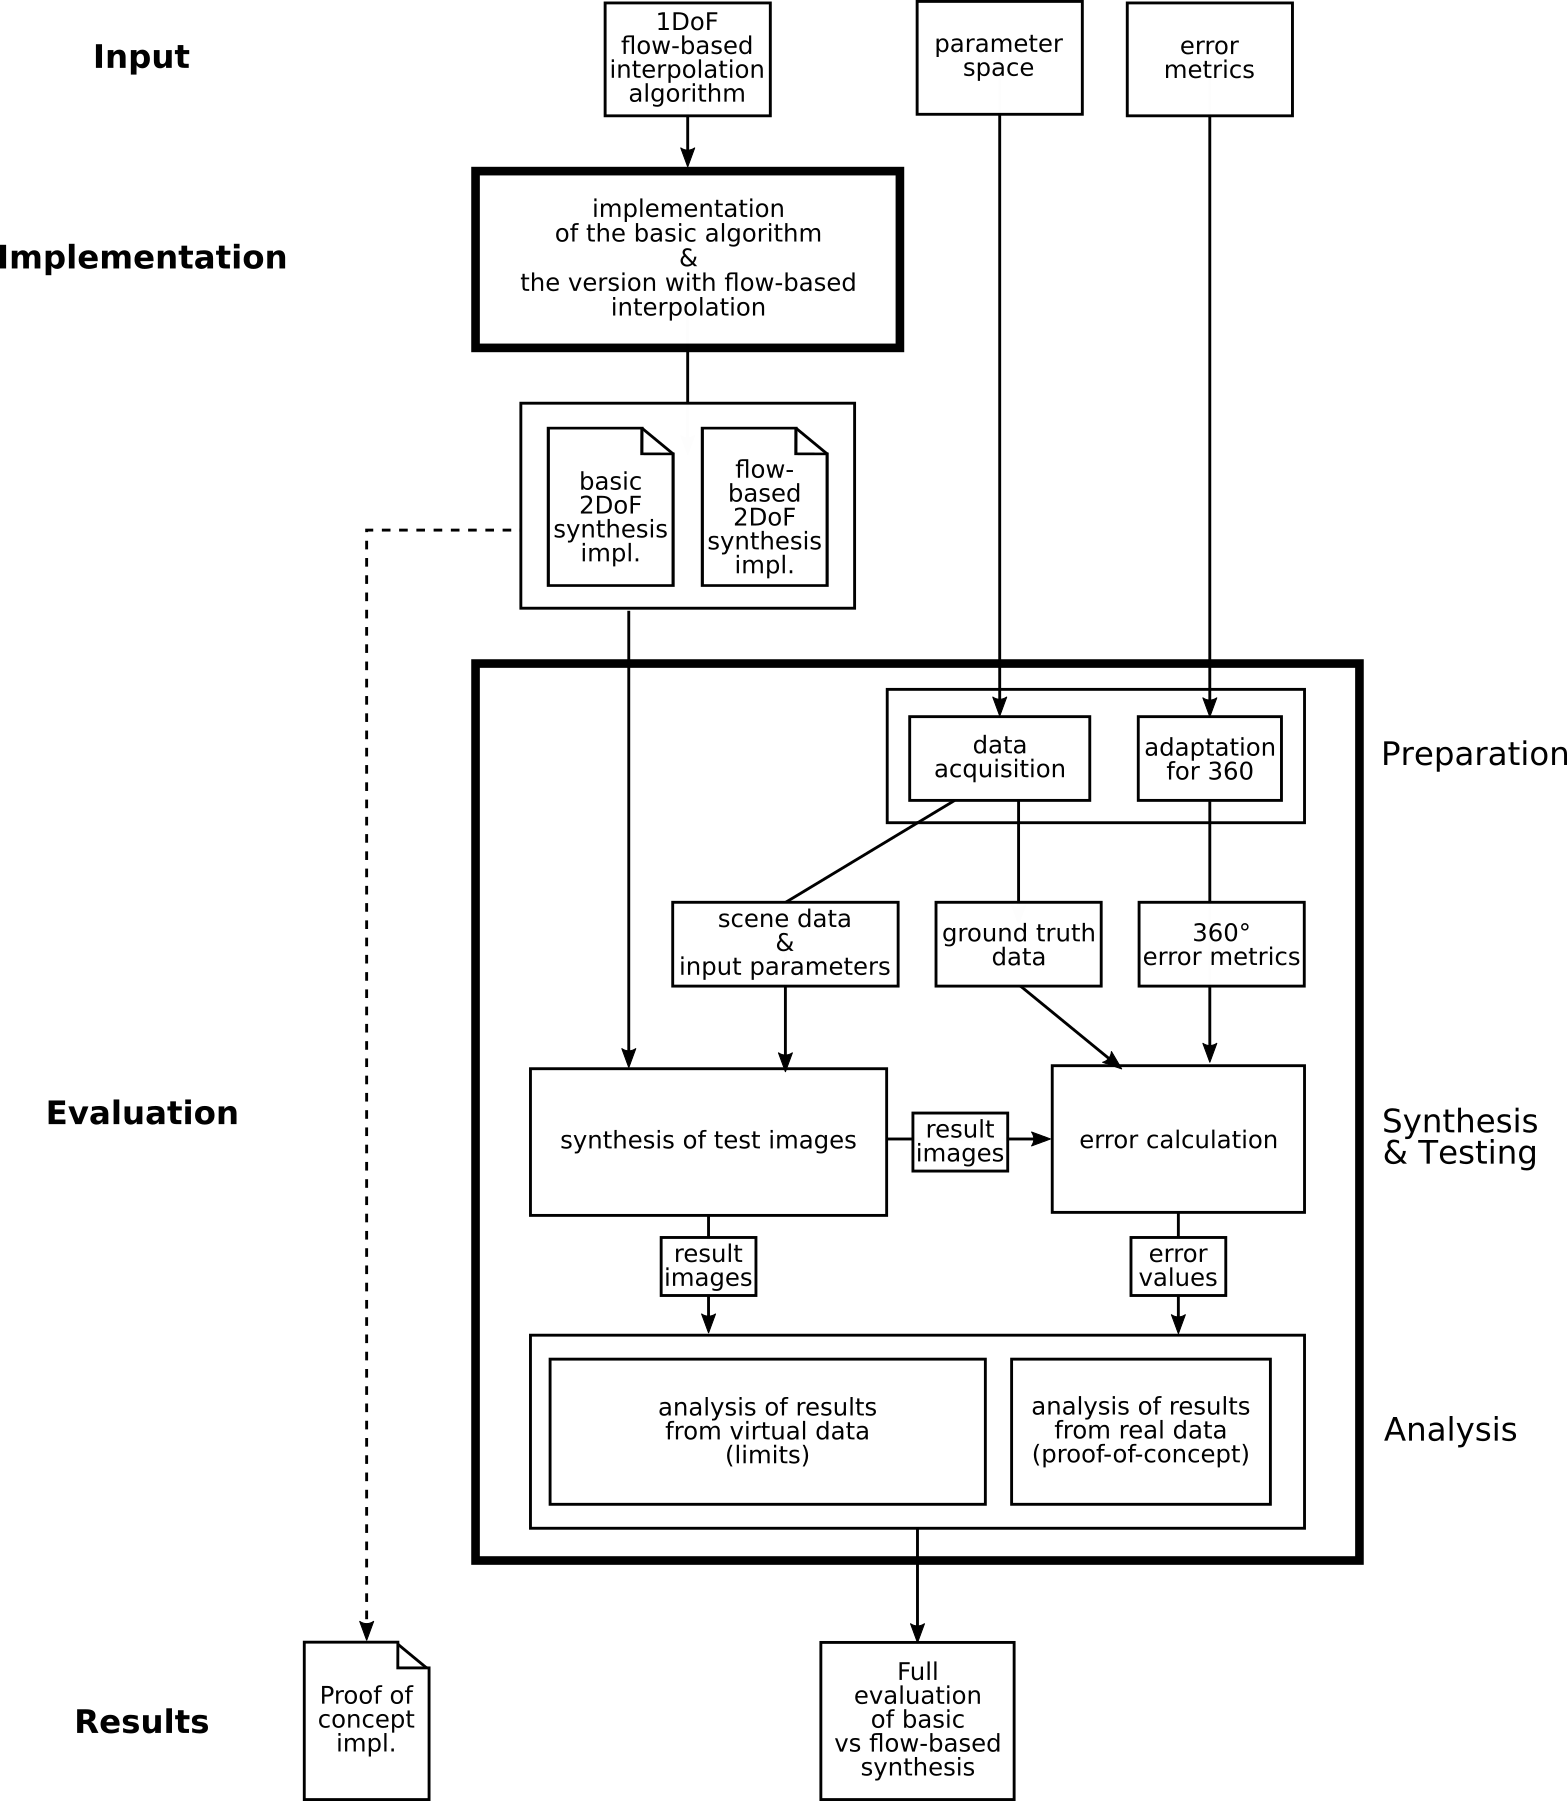
\includegraphics[width=0.9\textwidth]{01/methodology.png}
		\caption{Methodology}
		\label{fig:methodology}
\end{figure}

\section*{Results}
The results of this thesis are:
\begin{itemize}
  \item A basic proof-of-concept implementation of a 2DoF pixel-based synthesis algorithm with flow-based interpolation
  \item An evaluation of the results of this algorithm with a comparison of the pixel-based algorithm by itself versus with flow-based interpolation, proving that flow-based interpolation does improve the results of the basic algorithm in the majority of the examined cases
%  \item evaluation methodology for 360\degree images, including models and samples that can be used for benchmarking other methods \ar is it better than a naive algorithm?
\end{itemize}

The results of this thesis can be the basis of various future work. Since the implementation is a first attempt at combining the two methods, the problems and limitations discovered in the evaluation can be used to improve future versions. Alternative proxy geometries could be examined, potentially based on sparse scene geometry, which would improve the basic results and could lead to a distinct improvement of the flow-based results. Furthermore, parallelization and optimization could be used in order to achieve real-time framerates. 

%- proof of concept implementation
%- evaluation of flow-based vs regular with several select parameters
%- yes, in the majority of evaluated cases, flow-based blending brings an improvement (given the optical flow algorithm produces accurate results)
%- but also has several major drawbacks that need to be handled

%national park:
%https://www.oculus.com/experiences/go/1524331530931445/?ranking_trace=0_1524331530931445_SKYLINEWEB_D8RtWgI7mmWKB0QLB
%mecca
%https://www.oculus.com/experiences/go/1125286047502859/?ranking_trace=0_1125286047502859_SKYLINEWEB_1QYbs8B1KfddDpRhA

%Along with this development, 360\degree cameras (i.e.\ cameras that capture the complete surroundings) have become more consumer-friendly and affordable as well. Previously, capturing a true 360\degree image was a fairly laborious. Several regular images that had been captured meticulously with a single camera facing in different directions, or a state-of-the art camera with several lenses, had to be stitched together in software. However, recently, development of designated 360\degree cameras with several built-in lenses and integrated stitching, has led to an increase in popularity with consumers\footnote{The price of a consumer-quality 360\degree camera is between approximately 200 and 1000 USD as of January 2021 (\url{https://www.techradar.com/news/best-360-degree-camera}, \emph{accessed 13/1/21}}.

%Given these developments, it stands to reason that using 360\degree cameras to create immersive viewing experiences for VR is a next logical step. In fact,
